\section{Database}
\label{sec:database}

The \textit{viaappiadb} database is running in the Via Appia Linux server. See Section \ref{sec:software} on how to get an account in the database.

This database (DB) has conceptually two major parts and five categories: (a.) data management information and (b.) the attribute data. The  data management part has  4 categories: ITEM, RAW, POTREE and OSG and the attribute data are represented in category ATTRIBUTE.
 
In Figure \ref{fig:db_erdb} the Entity-Relationship diagram (ERD) of the \textit{viaappiadb} is shown. In next Subsections each category is described briefly and illustrated with its part of the ERD also indicating the connections (only direct links are indicated) to the other categories. 

Note that some of the nodes of the relationships are \textit{0:n} or \textit{0:1} (with black points) instead of the usual \textit{1:n} or \textit{1:1}. This is to illustrate that some sites and objects may have entries in some tables but not in others. For example it is possible to have a site in the item table which has no entry in the attributes table (tbl1\_site).

\begin{figure}[H]
\centering
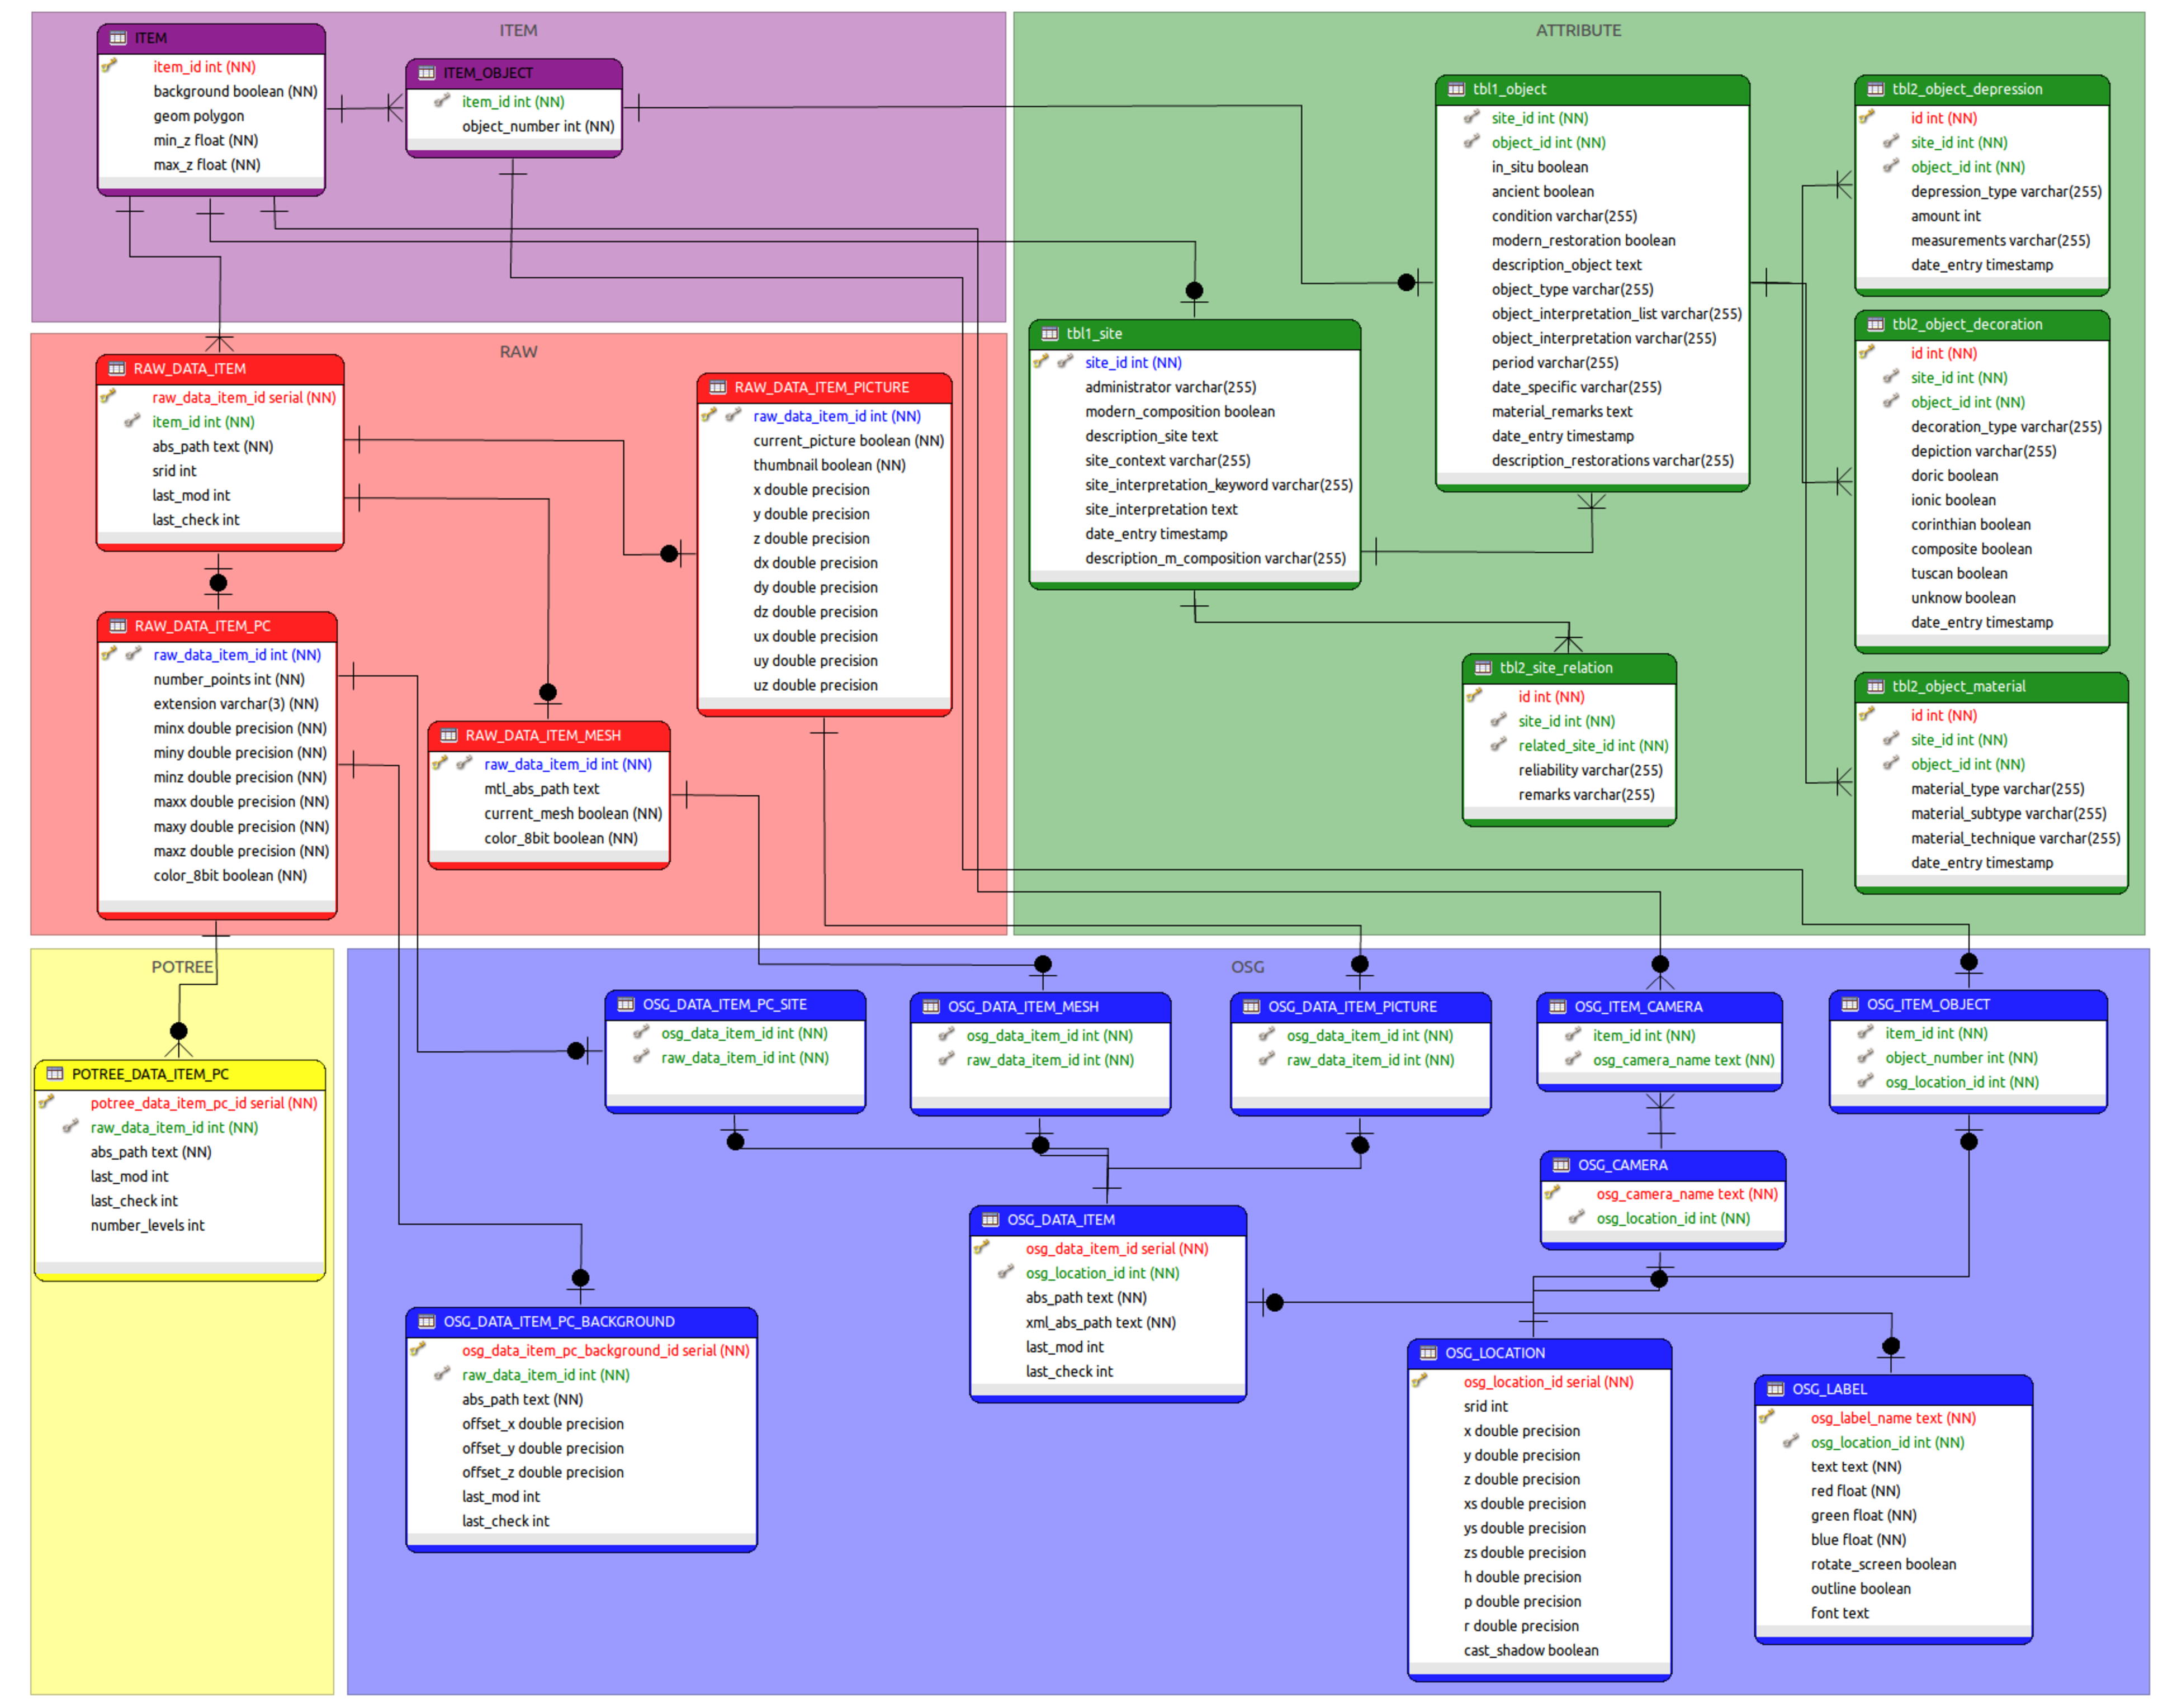
\includegraphics[scale=0.25]{fig/database/ERDB.pdf}
\caption{Entity-Relationship diagram of the \textit{viaappiadb} database with its five categories.}
\label{fig:db_erdb}
\end{figure}

\subsection {Data management}
This part of the DB contains tables with the locations of the raw and converted data, visualization-related data and the footprints (geometries) of the sites.

\subsubsection{ITEM}
Conceptually this is a category containing an information about an {\em item}. Item is any entity of interest- background (then the logical field {\em background} is set to true (1)) or site (0). Is the item of interest is an archaeological site (monument) it can contain one or more objects (parts of the site) which is reflected by the field {\em object\_numer}. Figure \ref{fig:db_erdb_item} shows the relationship of the ITEM category with the other categories. The ITEM category is on the top of the categories' hierarchy.
\begin{figure}[H]
\centering
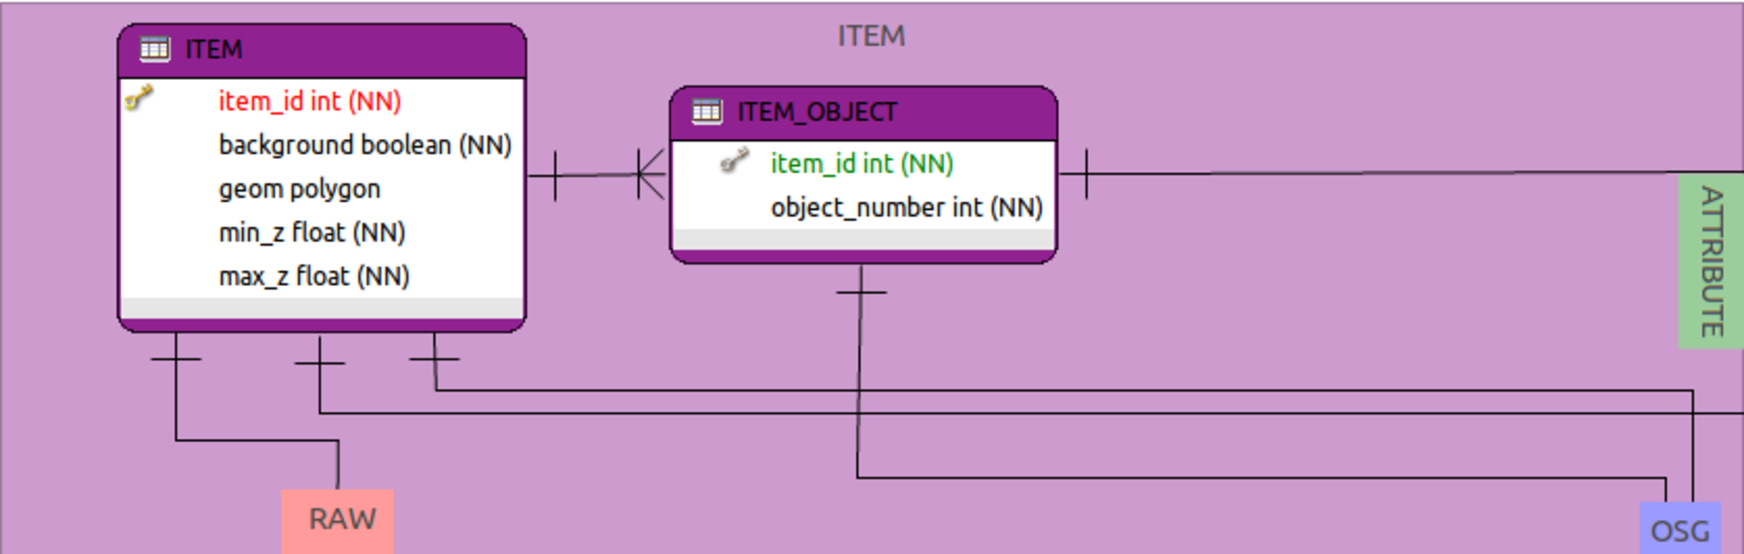
\includegraphics[scale=0.35]{fig/database/ERDB_ITEM_conn.pdf}
\caption{Entity-Relationship diagram of category ITEM and indicated connections with other categories.}
\label{fig:db_erdb_item}
\end{figure}

\subsubsection{RAW}
The RAW category contains all the \textit{raw data} gathered for given item. The most important meta-data is the location in the Data structure (Section \ref{sec:data_structure}), stored in the {\em abs\_path} field. These data can be either point clouds (PC), meshes (MESH) or pictures (PICTURE). Each of these types is represented by a separate table with the specific for that data type properties. The RAW category is related to the derived data categories OSG and POTREE as indicated on Figure \ref{fig:db_erdb_raw}. 
\begin{figure}[H]
\centering
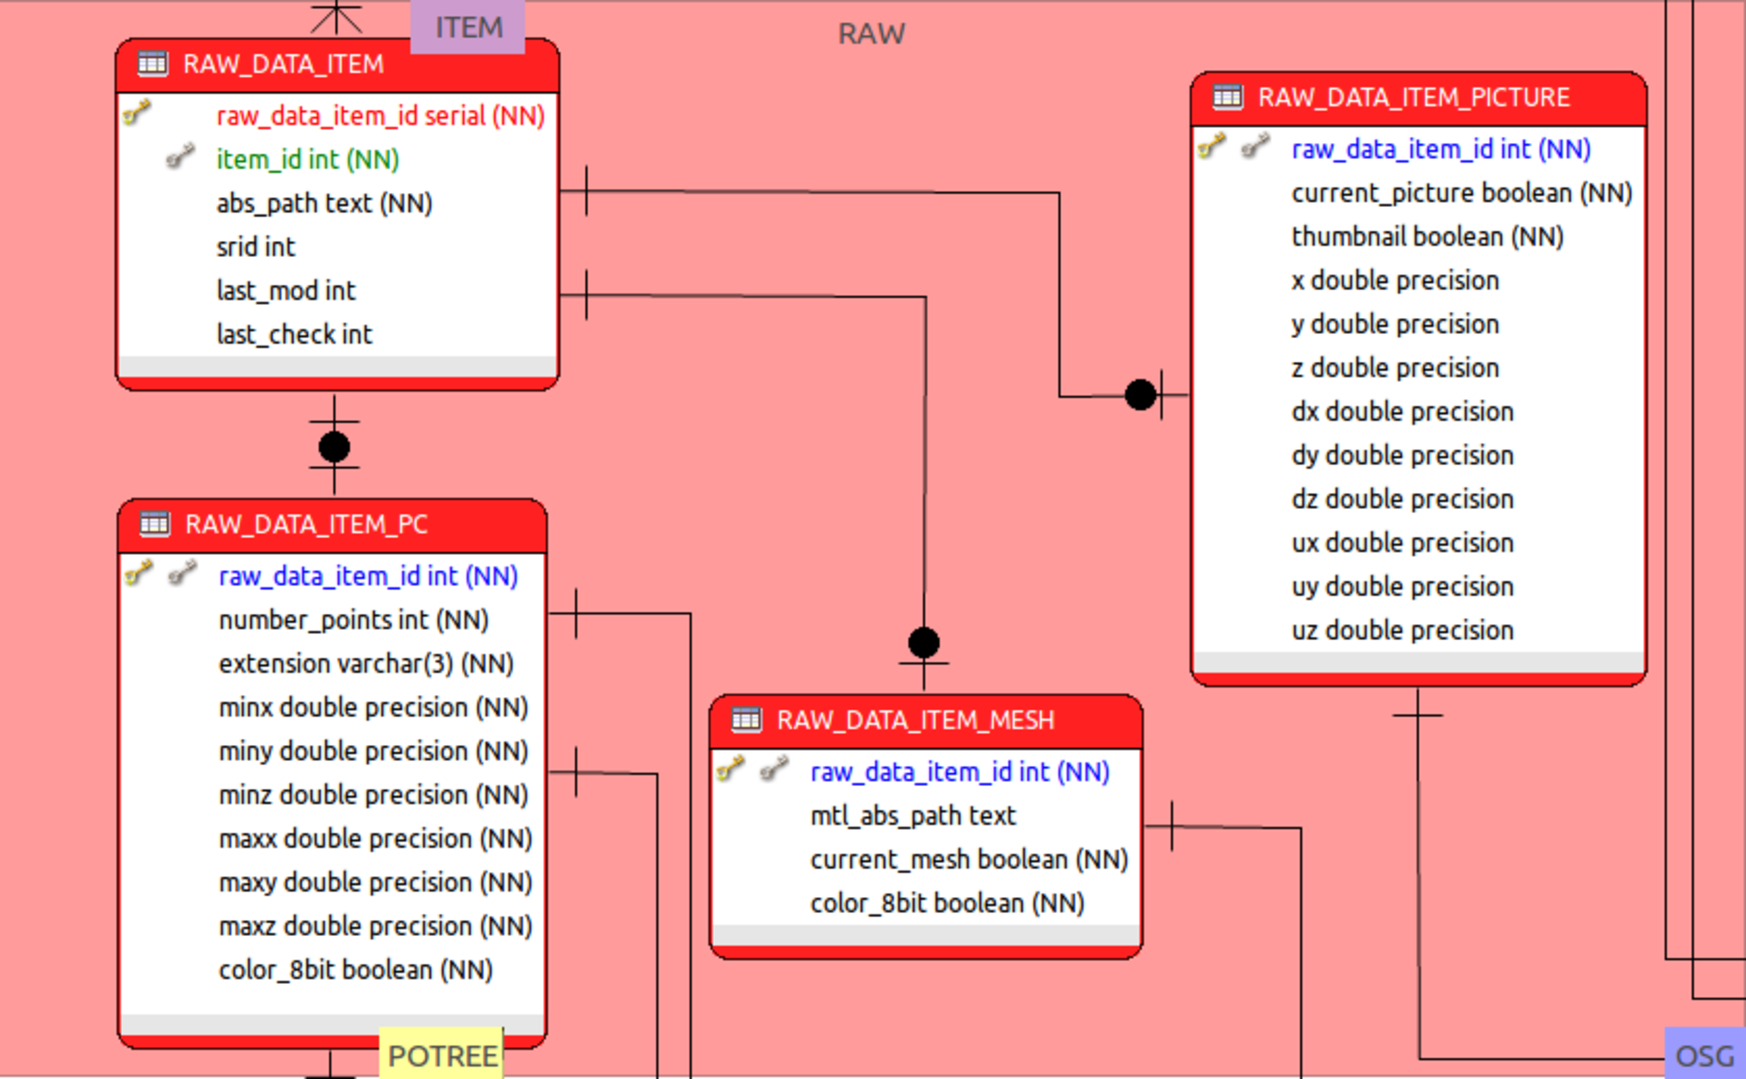
\includegraphics[scale=0.35]{fig/database/ERDB_RAW_conn.pdf}
\caption{Entity-Relationship diagram of category RAW and indicated connections with other categories.}
\label{fig:db_erdb_raw}
\end{figure}

\subsubsection{OSG}
This category represents the OSG \textit{converted data} used for the Windows desktop/laptop client application. As seen by the ERD on Figure \ref{fig:db_erdb_osg} it is related to the RAW data (from where it is derived) and to the ITEM category. The tables in this category reflect the possible data types: PC, meshes and pictures. Most importantly, this category contains information needed for the \textit{visualization}, like specifics of the background and items, the camera, location (bounding box) and label. 

\begin{figure}[H]
\centering
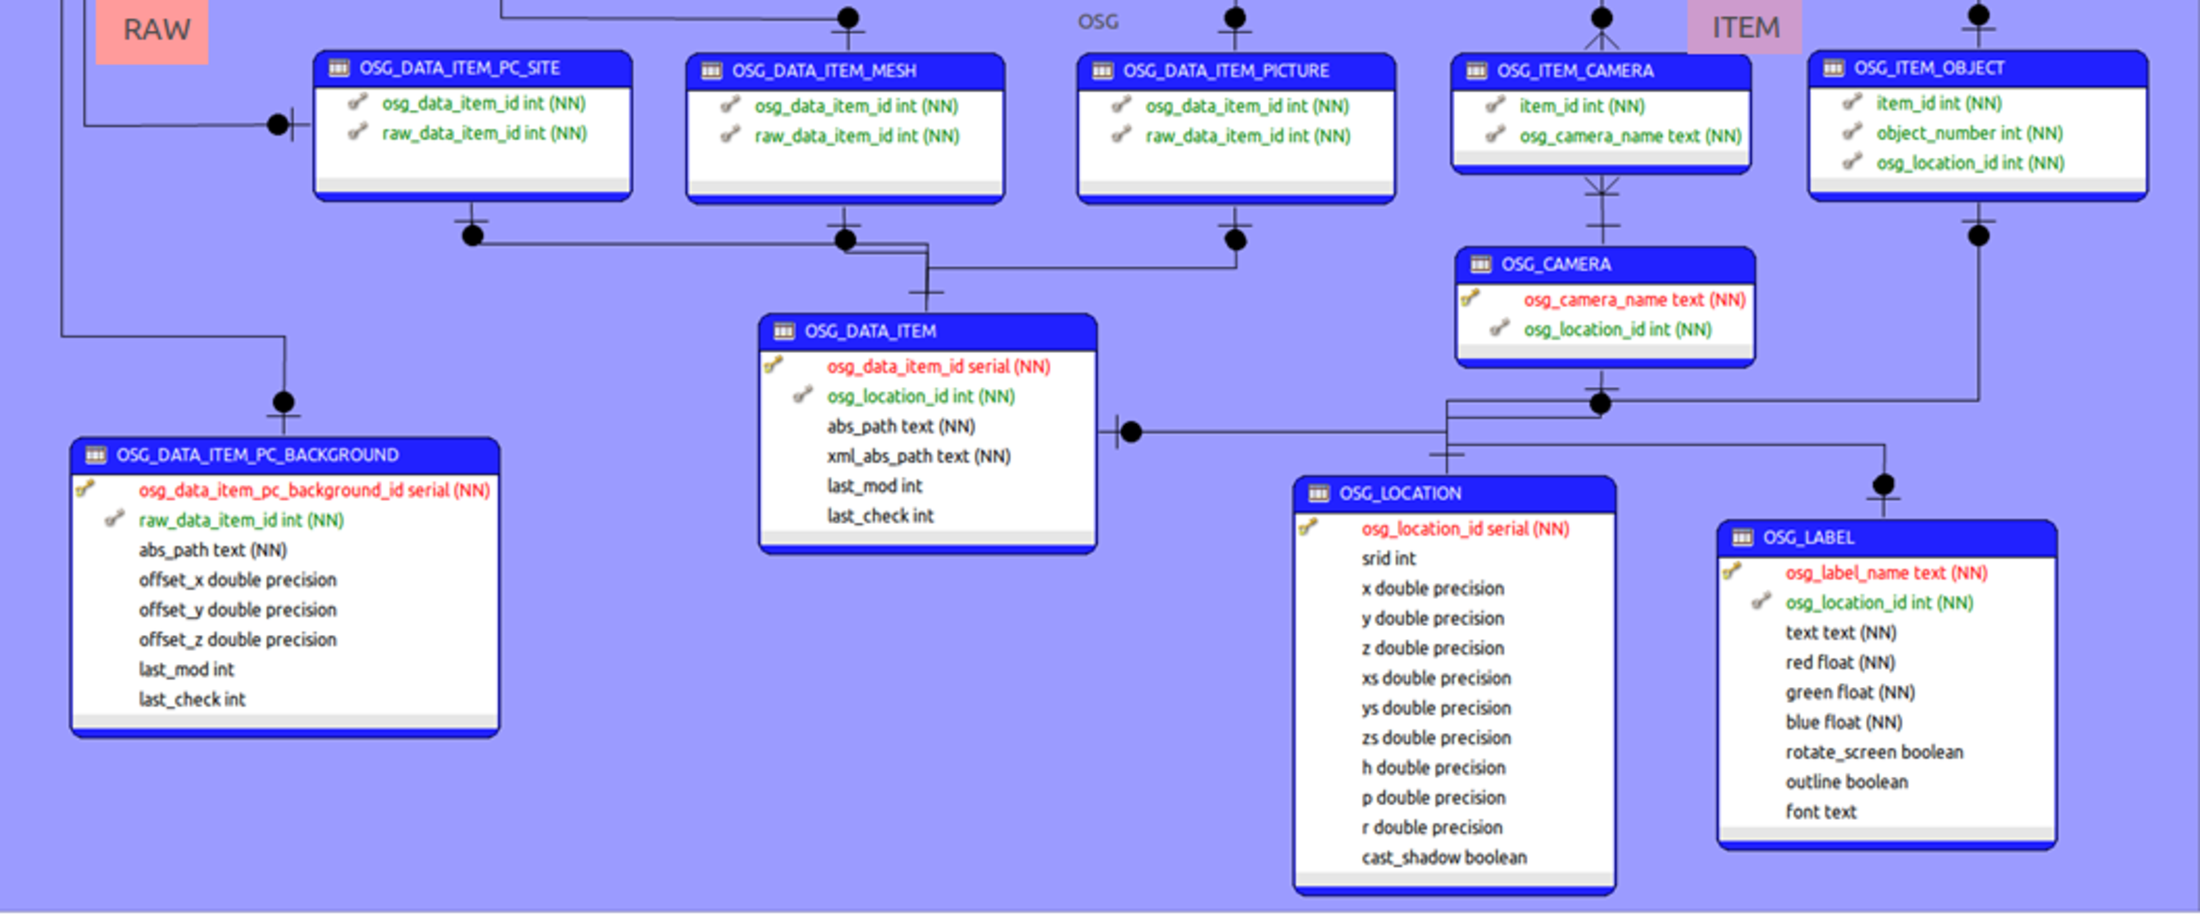
\includegraphics[scale=0.35]{fig/database/ERDB_OSG_conn.pdf}
\caption{Entity-Relationship diagram of category OSG and indicated connections with other categories.}
\label{fig:db_erdb_osg}
\end{figure}


\subsubsection{POTREE}
This category is illustrated on Figure \ref{fig:db_erdb_potree}. As it can be seen, it is related only to the RAW category from which it is derived using the POTREE converter and stores only data of the PC type and conversion parameters ({\em number_levels}).
\begin{figure}[!H]
\centering
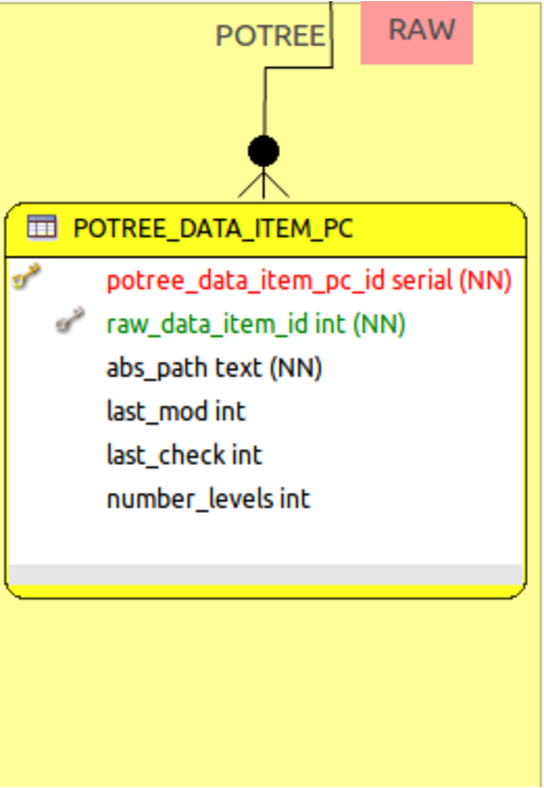
\includegraphics[scale=0.35]{fig/database/ERDB_POTREE_conn.pdf}
\caption{Entity-Relationship diagram of category POTREE and indicated connections with other categories.}
\label{fig:db_erdb_potree}
\end{figure}

\subsection{Attribute data}
The attribute part of the DB is represented only by one category (Figure \ref{fig:db_erdb_attribute}). It  is connected only to the ITEM category. These are the meta-data collected during the field work and are primarily of research interest to the archaeologists as it contains all domain-related data enabling browsing and filtering of sub-parts of the data of interest.

\begin{figure}[H]
\centering
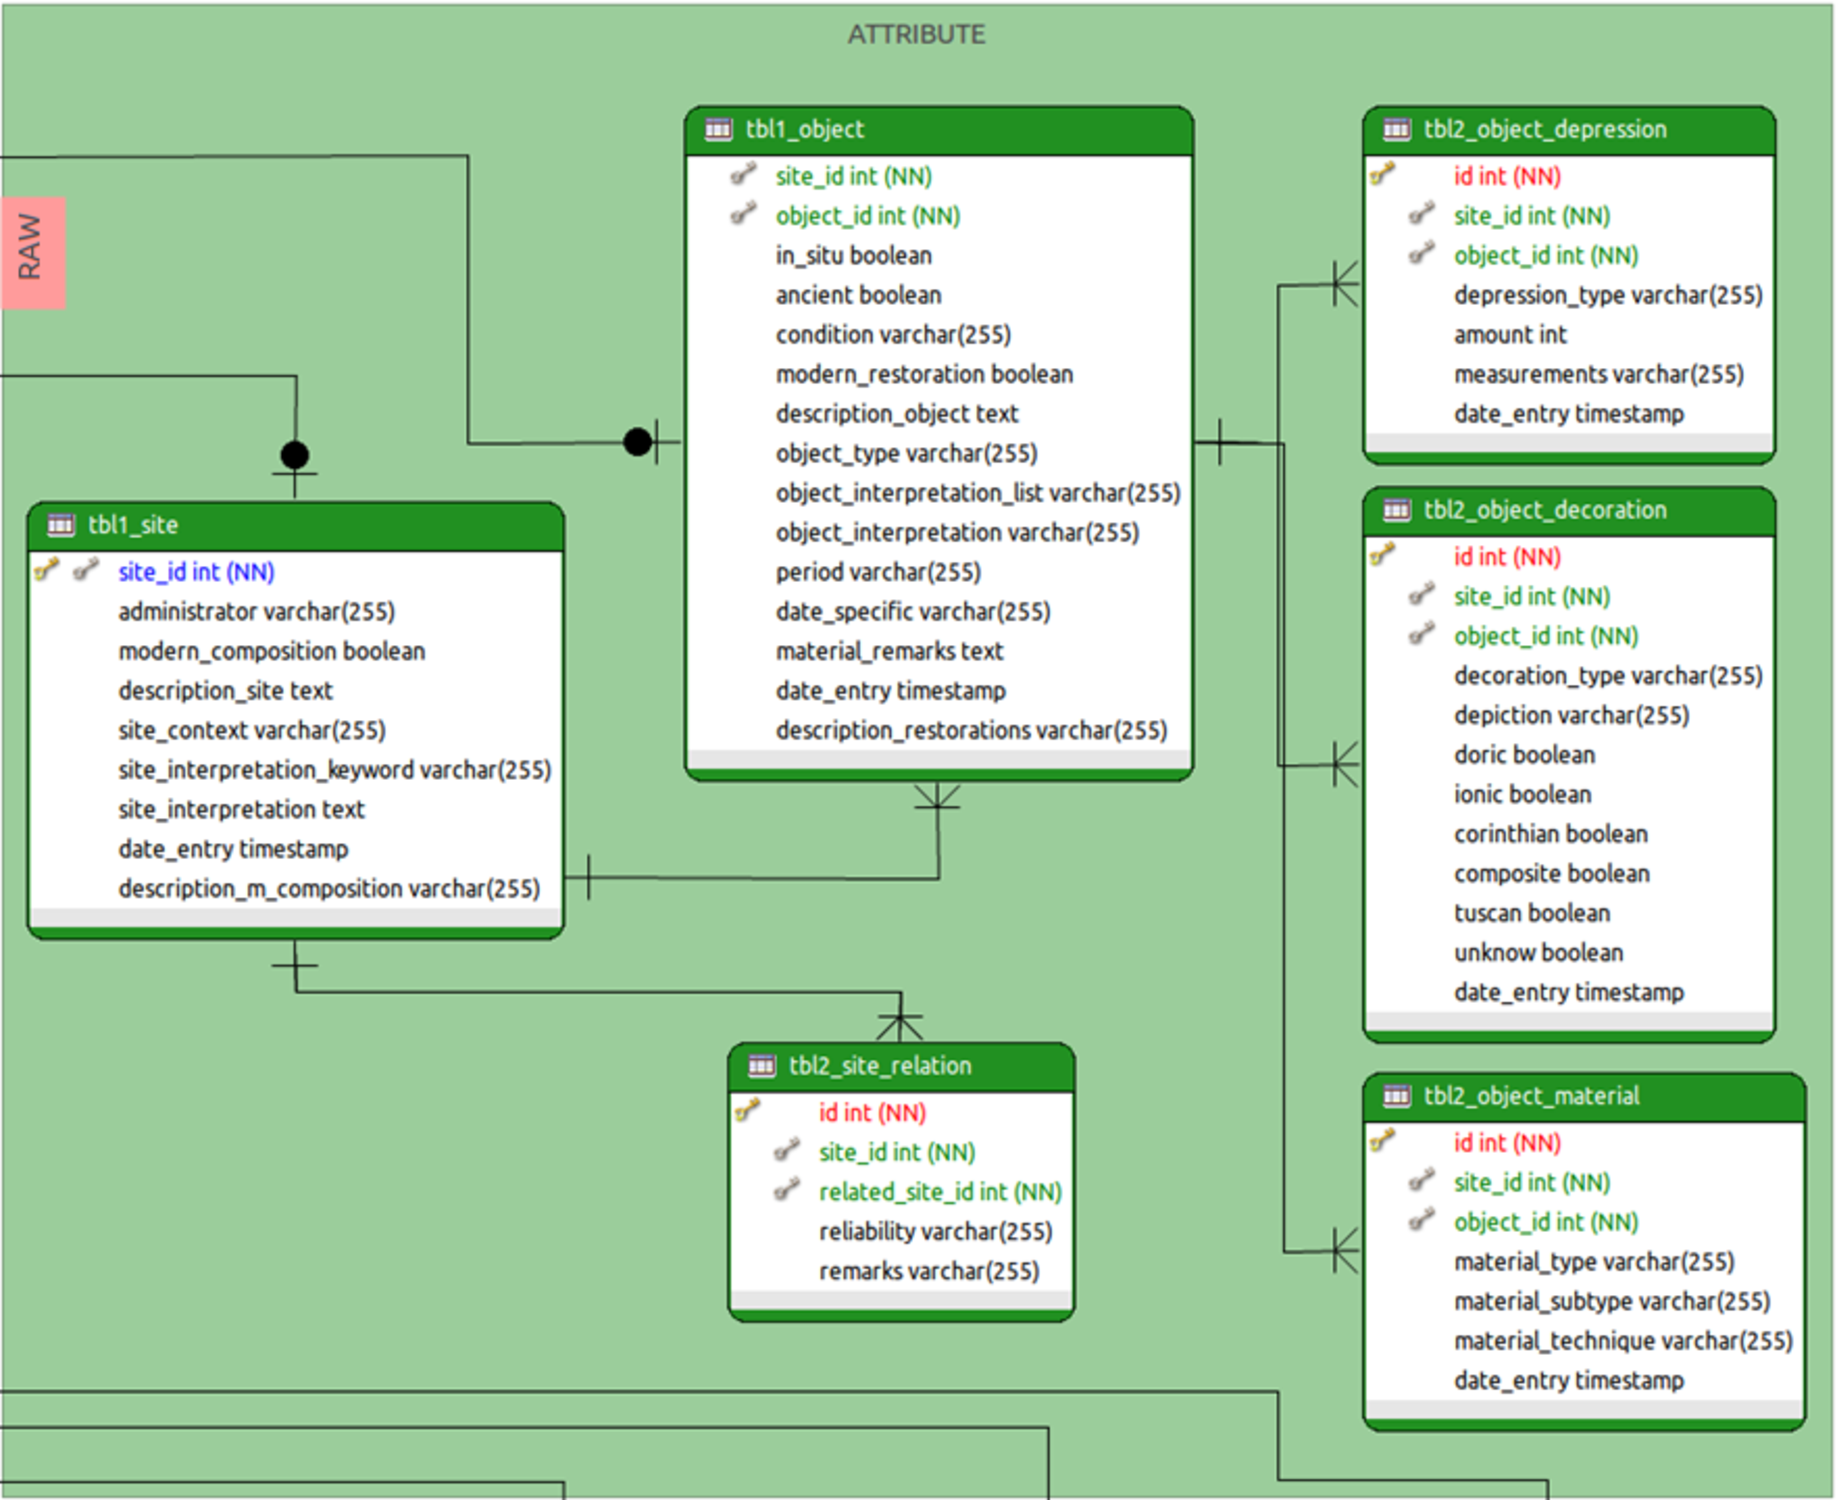
\includegraphics[scale=0.35]{fig/database/ERDB_ATTRIBUTE_conn.pdf}
\caption{Entity-Relationship diagram of category  ATTRIBUTE and indicated connections with other categories.}
\label{fig:db_erdb_attribute}
\end{figure}